\documentclass[10pt]{article}
\usepackage{fullpage}
\usepackage{amsmath}
\usepackage[amsthm, thmmarks]{ntheorem}
\usepackage{amssymb}
\usepackage{graphicx}
\usepackage{enumerate}
\usepackage{verse}
\usepackage{tikz}
\usepackage{verbatim}
\usepackage{hyperref}
\usepackage{bbm}

\newtheorem{lemma}{Lemma}
\newtheorem{theorem}[lemma]{Theorem}
\newtheorem{definition}[lemma]{Definition}
\newtheorem{proposition}[lemma]{Proposition}
\newtheorem{corollary}[lemma]{Corollary}
\newtheorem{claim}[lemma]{Claim}
\newtheorem{example}[lemma]{Example}

\newcommand{\dee}{\mathrm{d}}
\newcommand{\Dee}{\mathrm{D}}
\newcommand{\In}{\mathrm{in}}
\newcommand{\Out}{\mathrm{out}}
\newcommand{\pdf}{\mathrm{pdf}}
\newcommand{\Cov}{\mathrm{Cov}}
\newcommand{\Var}{\mathrm{Var}}

\newcommand{\ve}[1]{\mathbf{#1}}
\newcommand{\ves}[1]{\boldsymbol{#1}}
\newcommand{\mrm}[1]{\mathrm{#1}}
\newcommand{\etal}{{et~al.}}
\newcommand{\sphere}{\mathbb{S}^2}
\newcommand{\modeint}{\mathcal{M}}
\newcommand{\azimint}{\mathcal{N}}
\newcommand{\ra}{\rightarrow}
\newcommand{\mcal}[1]{\mathcal{#1}}
\newcommand{\X}{\mathcal{X}}
\newcommand{\Y}{\mathcal{Y}}
\newcommand{\Z}{\mathcal{Z}}
\newcommand{\x}{\mathbf{x}}
\newcommand{\y}{\mathbf{y}}
\newcommand{\z}{\mathbf{z}}
\newcommand{\tr}{\mathrm{tr}}
\newcommand{\sgn}{\mathrm{sgn}}
\newcommand{\diag}{\mathrm{diag}}
\newcommand{\Real}{\mathbb{R}}
\newcommand{\sseq}{\subseteq}
\newcommand{\ov}[1]{\overline{#1}}
\newcommand{\data}{\mathrm{data}}
\newcommand{\mtt}[1]{\mathtt{#1}}

\DeclareMathOperator*{\argmin}{arg\,min}


\title{Deformation Transfer for Triangle Meshes}
\author{Pramook Khungurn}

\begin{document}
\maketitle

This note is written as I read the ``deformation transfer for triangle meshes'' paper by Sumner and Popovic \cite{Sumner:2004}. This is a classic paper that starts the whole field of deformation transfer \cite{Roberts:2021:Survey}.

\section{Introduction}

\begin{itemize}
    \item The input has three triangular meshes.
    \begin{itemize}
        \item The \emph{source} mesh $S$.
        \item The \emph{deformed source} mesh $\widetilde{S}$.
        \item The \emph{target} mesh $T$.
    \end{itemize}
    
    \item The constraint between the input meshes is that $S$ and $\widetilde{S}$ should have the same topology: same number of vertices and triangles. The target mesh does not have to have the same topology.
    
    \item We want to create a new triangular mesh $\widetilde{T}$ that has the same topology as $T$. We want $\widetilde{T}$ to be $T$ with the same global, continuous, deformation of shape that was applied to get $\widetilde{S}$ from $S$.
    
    \item Some more notations.
    \begin{itemize}
        \item Let $S$ and $\widetilde{S}$ have $n$ vertices. 
        \item Let $|S|$ denote the number of triangles in $S$.
        \item Let us denote the vertices of $S$ by $\ve{v}_1, \ve{v}_2, \ldots, \ve{v}_n$.
        \item Let us denote the vertices of $\widetilde{S}$ by $\widetilde{\ve{v}}_1, \widetilde{\ve{v}}_2, \ldots, \widetilde{\ve{v}}_n$.
        \item Let $T$ and $\widetilde{T}$ have $m$ vertices.
        \item Let $|T|$ denote the number of triangles in $T$.
        \item Let us denote the vertices of $T$ by $\ve{t}_1, \ve{t}_2, \ldots, \ve{t}_m$.
        \item Let us denote the vertices of $\widetilde{T}$ by $\widetilde{\ve{t}}_1, \widetilde{\ve{t}}_2, \ldots, \widetilde{\ve{t}}_m$.
    \end{itemize}
     
    
    \item To take into account the differences between topology of $S$ and $T$, the user supplies a mapping $M$ between the source and the target triangles.
    \begin{align*}
        M = \{(s_1, t_1), (s_2, t_2), \ldots, (s_{|M|}, t_{|M|})\}.
    \end{align*}
    A pair $(s_i, t_i)$ means that the target triangle with index $t_i$ should deform like the source triangle with index $s_i$.

    \item In general, $M$ is a many-to-one mapping.
    
    \item Creating the mapping $M$ is a tedious task if it were to be done manually. The paper proposes a method to create it semi-automatically. We will talk about it later.
\end{itemize}

\section{First Formulation}

\begin{itemize}
    \item The \emph{source deformation} that gets us from $S$ to $\widetilde{S}$ is a collection of affine transformations tabulated for each triangle in $S$.
    
    \begin{itemize}
        \item We cannot compute this affine transformation from the vertex positions of the triangles in $S$ and $\widetilde{S}$. This is because the changes in vertex positions do not determine how the space perpendicular to the triangle deforms.
        
        \item To resolve the problem, we add a fourth vertex in the direction perpendicular to the triangle. Let $\ve{v}_1$, $\ve{v}_2$, and $\ve{v}_3$ be the vertices of the triangle in $S$. The fourth vertex $\ve{v}_4$ is given by:
        \begin{align*}
            \ve{v}_4 = \ve{v}_1 + \frac{(\ve{v}_2 - \ve{v}_1) \times (\ve{v}_3 - \ve{v}_1)}{\sqrt{\| (\ve{v}_2 - \ve{v}_1) \times (\ve{v}_3 - \ve{v}_1) \|}}.
        \end{align*}
        We also perform the same computation for the vertices $\widetilde{\ve{v}}_1$, $\widetilde{\ve{v}}_2$, and $\widetilde{\ve{v}}_3$ in $\widetilde{S}$.

        \item Note that the vector that we add to $\ve{v}_1$ to get $\ve{v}_4$ is not a unit vector. Its length is proportional to the square root of the area of the triangle. It scales proportionally to the length of the triangle edges.
        
        \item The affine transformation is defined by a $3 \times 3$ matrix $Q$ and a displacement vector $\ve{d} \in \Real^3$. We will write it as $Q + \ve{d}$.
    
        \item We want the transformation to be so that
        \begin{align*}
            Q\ve{v}_i + \ve{d} = \widetilde{\ve{v}}_i
        \end{align*}        
        for $i = 1$, $2$, $3$, and $4$.
        
        \item If we subtract the first equation from the others, we have that
        \begin{align*}
            Q(\ve{v}_2 - \ve{v}_1) &= \widetilde{\ve{v}}_2 - \widetilde{\ve{v}}_1,\\
            Q(\ve{v}_3 - \ve{v}_1) &= \widetilde{\ve{v}}_3 - \widetilde{\ve{v}}_1,\\
            Q(\ve{v}_4 - \ve{v}_1) &= \widetilde{\ve{v}}_4 - \widetilde{\ve{v}}_1.
        \end{align*}
        Putting the above equations into a matrix, we have that
        \begin{align*}
            Q \begin{bmatrix}
                \ve{v}_2 - \ve{v}_1 &
                \ve{v}_3 - \ve{v}_1 &
                \ve{v}_4 - \ve{v}_1
            \end{bmatrix} 
            &= \begin{bmatrix}
                \widetilde{\ve{v}}_2 - \widetilde{\ve{v}}_1 &
                \widetilde{\ve{v}}_3 - \widetilde{\ve{v}}_1 &
                \widetilde{\ve{v}}_4 - \widetilde{\ve{v}}_1
            \end{bmatrix}.
        \end{align*}
        If we let
        \begin{align*}
            V &= \begin{bmatrix}
                \ve{v}_2 - \ve{v}_1 &
                \ve{v}_3 - \ve{v}_1 &
                \ve{v}_4 - \ve{v}_1
            \end{bmatrix}, \\
            \widetilde{V} &= \begin{bmatrix}
                \widetilde{\ve{v}}_2 - \widetilde{\ve{v}}_1 &
                \widetilde{\ve{v}}_3 - \widetilde{\ve{v}}_1 &
                \widetilde{\ve{v}}_4 - \widetilde{\ve{v}}_1
            \end{bmatrix},
        \end{align*}
        we have that
        \begin{align*}
            QV = \widetilde{V}.
        \end{align*}
        This gives us
        \begin{align*}
            Q = \widetilde{V} V^{-1}.
        \end{align*}
        
        \item Once we have $Q$, we can use it to solve for $\ve{d} = \widetilde{\ve{v}}_1 - Q\ve{v}_1$.
        
        \item For each triangle $j$, we compute $\mtt{S}_j = Q_j + \ve{d}_j$ for $j = 1, 2, \ldots, |S|$.
    \end{itemize}

    \item Let's try to understand the effect of the source transformation on the target mesh, assuming that we already have the mapping in place.
    \begin{itemize}
        \item First, let's get ourselves the source mesh (top left), the deformed source mesh (bottom left), and the target mesh (top right). \\
        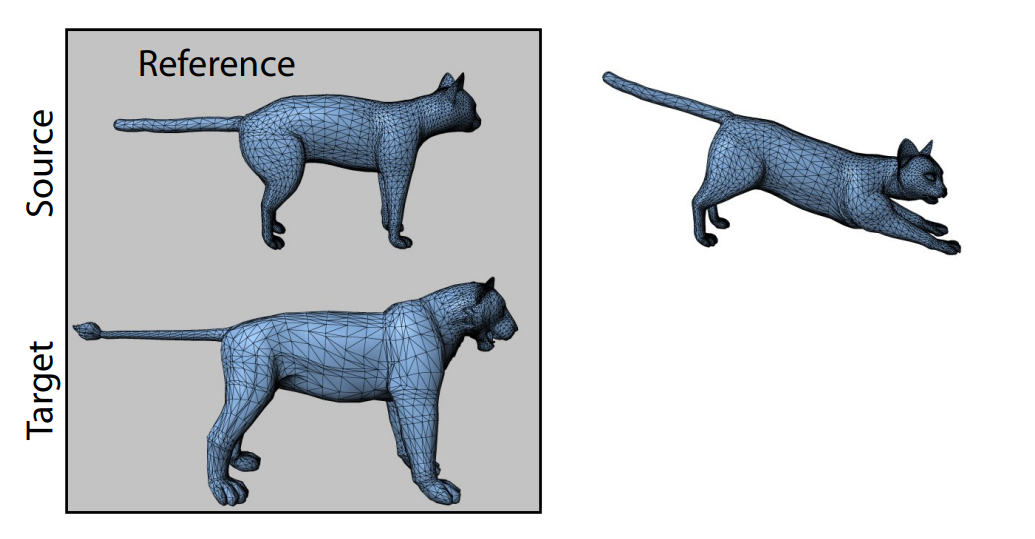
\includegraphics[width=0.5\textwidth]{images/deformation-transfer-inputs.png}

        \item If we apply only the linear part of the source deformation, $Q_j$, to the target triangles, we get something like this. \\
        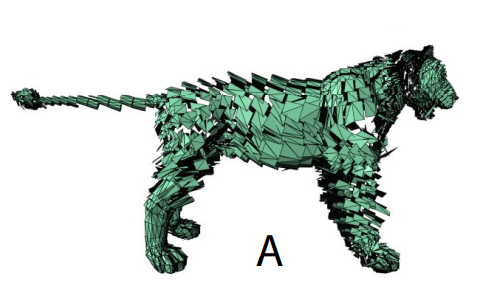
\includegraphics[width=0.5\textwidth]{images/deformation-transfer-step-1.png}\\
        We see here that the triangles in the target mesh change their orientations and sizes, but the positions are not changed. (Recall that everything is anchored to $\ve{v}_1$.)

        \item If we also apply the translation $\ve{d}_j$ to the target triangles as well, we get something like this. \\
        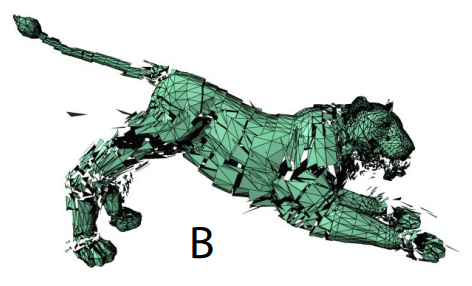
\includegraphics[width=0.5\textwidth]{images/deformation-transfer-step-2.png}\\
        We see that the triangles also change their positions. However, the mesh is no longer connected.
    \end{itemize}

    \item So, in order not to tear up the target mesh, we need to make sure that the triangles are connected after transformations.
    \begin{itemize}
        \item Let us say that the target deformation is $\mtt{T}_j = R_j + \ve{e}_j$ for $j = 1, 2, \ldots, |T|$.
        \begin{itemize}
            \item Here, $R_j$ is the analogue of $Q_j$, and $\ve{e}_j$ is the analogue of $\ve{d}_j$.
        \end{itemize}
    
        \item We require that shared vertices be transformed to the same position. In other words, let $\ve{w}_i$ be a vertex in the target mesh, and let $p(\ve{w}_i)$ be the set of triangles that contains $\ve{w}_i$. We require that
        \begin{align*}
            R_j \ve{w}_i + \ve{e}_j = R_k \ve{w}_i + \ve{e}_k
        \end{align*}
        for all $j, k \in p(\ve{w}_i)$.
    \end{itemize}

    \item Deformation transfers solve an optimization problem to make the target deformation as close as possible to the source deformation while maintaining the connectedness above.
    \begin{align*}
        & \min_{\mtt{T}_1, \mtt{T}_2, \ldots, \mtt{T}_{|T|}} \sum_{j=1}^{|M|} \| \mtt{T}_{t_j} - \mtt{S}_{s_j} \|^2_F \\
        & \mbox{subject to: } R_j \ve{w}_i + \ve{e}_j = R_k \ve{w}_i + \ve{e}_k \mbox{ for all } j, k \in p(\ve{w}_i) \mbox{ for all vertices } \ve{w}_i.
    \end{align*}
    Recall that $\mtt{S}_{s_j}$ and $\mtt{T}_{t_j}$ are affine transformations in 3D, and this means that they can be represented by $4 \times 4$ matrices. So, the Frobenius norm of the difference between the two is well defined.
\end{itemize}

\section{Vertex Formulation}

\begin{itemize}
    \item The above formulation is a constrained quadratic optimization problem with linear constraints. While this is a convex optimization problem that has a solution, it is inefficient. (Honestly, I also don't know how to do it myself.)
    
    \item There is a much better formulation that casts the problem in terms of the output vertex positions.
    \begin{itemize}
        \item We define the target deformation in terms of the output vertex positions.
        \item We solve directly for the output vertex positions so as to minimize the difference between the source and the target deformations.
    \end{itemize}

    \item To do this, for each target triangle, we add a fourth vertex. Then, we have that
    \begin{align*}
        R = \widetilde{W} W^{-1}.
    \end{align*}
    \begin{itemize}
        \item The elements of $W^{-1}$ are known: they are the vertices of the target mesh. 
        \item The elements of $\widetilde{W}$ are unknown: they are the vertices of the deformed target mesh. 
        \item So, the elements of $R$ are linear combinations of the coordinates of the unknown deformed vertices.
    \end{itemize}
    
    \item With the above identity, we can rewrite the minimization problem as follows:    
    \begin{align*}
        \min_{\widetilde{\ve{w}}_1, \widetilde{\ve{w}}_2, \ldots, \widetilde{\ve{w}}_m} 
        \sum_{j=1}^{|M|} \| \mtt{T}_{t_j} - \mtt{S}_{s_j}  \|_F^2
    \end{align*}

    \item We can rewrite the above minimization problem as a least squares problem.
    \begin{align*}
        \min_{\widetilde{\ve{w}}_1, \widetilde{\ve{w}}_2, \ldots, \widetilde{\ve{w}}_m} 
        \| \ve{c} - A\widetilde{\ve{w}} \|_2^2.
    \end{align*}
    Here:
    \begin{itemize}
        \item $\widetilde{\ve{w}}$ is the big vector of unknown deformed vertex positions.
        \item $\ve{c}$ is a vector containing entries from the source transformations.
        \item $A$ is a large matrix that relates $\widetilde{\ve{w}}$ to $\ve{c}$.
    \end{itemize}
    The optimal solution is given by
    \begin{align*}
        \widetilde{\ve{w}} = (A^T A)^{\dagger} A^T \ve{c},
    \end{align*}
    which is standard knowledge.

    \item In practice, we need to compute $A$. Then, we can factor $A^T A$ so that it becomes easy to invert, like with an LU or a Cholesky factorization or something like that. Then, we can solve for $\widetilde{\ve{w}}$.
\end{itemize}

\section{Correspondence}

\begin{itemize}
    \item We need to discuss how to determine $M$, the mapping between the source and the target triangles.
    
    \item For this, we need help from the user.
    \begin{itemize}
        \item The user selects $N$ pairs of source and target vertices that correspond to each other.
        \item Let us call these pairs $(a_1, b_1), (a_2, b_2), \ldots, (a_N, b_N)$.
        \item A pair $(a_i, b_i)$ indicates that the source vertex $\ve{v}_{a_i}$ should correspond to the target vertex $\ve{w}_{b_i}$.
    \end{itemize}

    \item The mapping is then computed with an iterated closest point algorithm with regularization.
    
    \item The algorithm performs the following steps:
    \begin{enumerate}
        \item It deforms the source mesh to the target mesh.
        \item It computes the triangle correspondence by searching for pairs of source and target triangles whose centroids are in close proximity.
    \end{enumerate}    

    \item To deform the source mesh to the target mesh, we solve a minimization problem that is similar to the one we used in the last section.
    
    \begin{itemize}
        \item However, the objective function is designed to deform one mesh \emph{into} the other rather than deforming it \emph{like} how the other deforms.
        
        \item A pair of corresponding vertices indicates that, after deformation, the source vertex should match the location of the target vertex. Each pair becomes an optimization constraint.
        
        \item The objective function also contains multiple terms.
        \begin{itemize}
            \item One that enforces deformation smoothness.
            \item One that prevents over smoothing.
            \item One that moves the source vertices to the target vertices.
        \end{itemize}
    \end{itemize}

    \item Let us set up the transformation problem.
    \begin{itemize}
        \item We wish to optimize the vertex positions of the deformed mesh $\widetilde{S}$ so that it is as close as possible to the target mesh $T$.
        \item The transformation we wish to optimize is $\mtt{S}_j = Q_j + \ve{d}_j$ for $j = 1, 2, \ldots, |S|$.
        \item Again, we have that
        \begin{align*}
            Q_j = \widetilde{V}_j V_j^{-1}.
        \end{align*}
        Here, $\widetilde{V}_i$ is unknown because it is a function of the unknown vertex positions of $\widetilde{S}$. On the other hand, $V_i$ is known because it is a function of the known vertex positions of $S$.
    \end{itemize}

    \item The \emph{deformation smoothness loss} $E_S$ requires that the transformations for adjacent triangles should be similar.
    \begin{align*}
        E_S = \sum_{j=1}^{|S|} \sum_{k \in \mathrm{adj}(j)} \| \mtt{S}_j - \mtt{S}_k \|^2_F
    \end{align*}
    where $\mathrm{adj}(j)$ is the set of triangles that are adjacent to triangle $j$.    

    \item The \emph{deformation identity loss} $E_I$ requires that all the transformations should be close to the identity transformation.
    \begin{align*}
        E_I = \sum_{j=1}^{|S|} \| \mtt{S}_j - I \|^2_F
    \end{align*}
    Its purpose is to prevent the deformation smoothness loss from generating a drastic change in the shape of the mesh in order to achieve optimal smoothness (such as collapsing the mesh into a single point).

    \item The \emph{closest valid point term} $E_C$ requires that the deformed source vertex should be equal to the closest valid point on the target mesh.
    \begin{align*}
        E_i = \sum_{i=1}^n \| \widetilde{\ve{v}}_i - \ve{c}_i \|^2.
    \end{align*}
    Here, $\ve{c}_i$ is the closest ``valid point'' on the target mesh to the deformed source vertex $\widetilde{\ve{v}}_i$.
    \begin{itemize}
        \item A point on the target mesh is considered ``valid'' for $\widetilde{\ve{v}}_i$ if its normal vector makes an angle of less than $90^\circ$ with the normal vector of $\widetilde{\ve{v}}_i$.
        
        \item A grid-based spatial sorting algorithm accelerates the closest point computation for this loss.
    \end{itemize}

    \item The optimization problem for correspondence is as follows.
    \begin{align*}
            &\min_{\widetilde{\ve{v}}_1, \widetilde{\ve{v}}_2, \ldots, \widetilde{\ve{v}}_n} \lambda_S E_S + \lambda_I E_I + \lambda_C E_C \\
            &\mbox{subject to: } \widetilde{\ve{v}}_{a_i} = \ve{w}_{b_i} \mbox{ for all } i = 1, 2, \ldots, N.
    \end{align*}
    Here, $\lambda_S$, $\lambda_I$, and $\lambda_C$ are weights of the loss terms.

    \item Note that the constraints basically reduce the number of unknowns, so it is a least-square problem with no constraints.

    \item The minimization problem is solved in two phases.
    \begin{itemize}
        \item In the first phase, we set $w_S = 1.0$, $w_I = 0.001$, and $w_C = 0.0$, ignoring the closest point term.
        \item In the second phase, we solve the same problem, increasing $w_C$ each time and updating the closest points after each iteration. The weights $w_S$ and $w_I$ remain the same, but $w_C$ is increased in four steps from $1.0$ to $5000.0$.
    \end{itemize}

    \item Once the source mesh has been deformed to the shape of the target mesh, we compute triangle correspondences by comparing the centroids of the deformed source and target triangles.
    \begin{itemize}
        \item Two triangles are ``compatible'' if the centroids are within a certain threshold of each other and the angle between their normals is less than $90^\circ$.
        
        \item For each triangle in the deformed source, we compute the closest compatible triangle in the target mesh, and add the pair to the mapping $M$.
        
        \item For each triangle in the target, we compute the closest compatible triangle in the deformed source mesh, and add the pair to the mapping $M$.
        
        \item A target triangle may correspond to multiple source triangles and vice versa.
    \end{itemize}
\end{itemize}

\section{Vertex Formulation Details}

\begin{itemize}
    \item To repeat optimization problem for the deformation transfer is as follows.
    \begin{align*}
        \min_{\widetilde{\ve{w}}_1, \widetilde{\ve{w}}_2, \ldots, \widetilde{\ve{w}}_m} 
        \| \ve{c} - A\widetilde{\ve{w}} \|_2^2.
    \end{align*}
    However, we didn't actually specify what these variables are.

    \item The first thing to consider that is how many unknowns are there. From the statement, it seems that there are $3m$ unknowns. However, this is not true.
    \begin{itemize}
        \item Remember that for each triangle in the deformed target mesh, we need to add a fourth vertex.
        \item We have seen so far that, in other $S$, $\widetilde{S}$, and $T$, the fourth vertex is a function of the three vertices of the triangle.
        \item However, the vertices of $\widetilde{T}$ are unknown. If we add a function of unknowns and compute with it, the problem becomes much more complicated to the extent that it cannot be casted as a least-squares problem.
        \item So, we need to add an unknonw point for each of the triangles instead.
        \item As a result, there are $3(m + |T|)$ unknowns.
        \item Therefore, $\widetilde{\ve{w}}$ is a vector of length $3(m + |T|)$.
    \end{itemize}

    \item Next, let's talk about $\ve{c}$. How many components that it has?
    \begin{itemize}
        \item Recall that $\| \ve{c} - A\widetilde{\ve{w}} \|_2^2$ is supposed to be equal to $\sum_{j=1}^{|M|} \| \mtt{T}_{t_j} - \mtt{S}_{s_j} \|^2_F$.
        
        \item As a result, there are $M$ pairs of matrices to compare.
    
        \item We have that $T_{t_j}$ and $S_{s_j}$ are $4 \times 4$ matrices. However, the 4th row is fixed to $(0, 0, 0, 1)$. So, we only need to compare the first three rows, which has 12 numbers.
        
        \item So, $\ve{c}$ has $12|M|$ components.
    \end{itemize}

    \item As result, $A$ is a $12|M| \times 3(m + |T|)$ matrix. This matrix is mostly sparse.
\end{itemize}

\section{Correspondence Details}

Note that material in this section is considered standard knowledge in optimization. However, I will include it here so that I have a nice reference when I implement stuffs.

\subsection{Combining Multiple Losses}

\begin{itemize}
    \item Suppose that we have a loss function that has multiple terms.
    \begin{align*}
        E = \sum_{i=1}^k \lambda_i E_i
    \end{align*}
    where each term $E_i$ is of the form
    \begin{align*}
        E_i = \| \ve{b}_i - A_i \ve{x} \|^2,
    \end{align*}
    and $\lambda_i$ are positive weights.
    
    \item We have that
    \begin{align*}
        E_i 
        &= (A_i \ve{x} - \ve{b}_i)^T (A_i \ve{x} - \ve{b}_i) \\
        &= \ve{x}^T A_i^T A_i \ve{x} - 2 \ve{x}^T A_i^T \ve{b}_i + \ve{b}_i^T \ve{b}_i.
    \end{align*}
    As a result,
    \begin{align*}
        E 
        &= \sum_{i=1}^k \lambda_i (\ve{x}^T A_i^T A_i \ve{x} - 2 \ve{x}^T A_i^T \ve{b}_i + \ve{b}_i^T \ve{b}_i) \\ 
        &= \ve{x}^T \left( \sum_{i=1}^k \lambda_i A_i^T A_i \right) \ve{x} - 2 \ve{x}^T \left( \sum_{i=1}^k \lambda_i  A_i^T \ve{b}_i \right) + \sum_{i=1}^k \lambda_i \ve{b}_i^T \ve{b}_i.
    \end{align*}
    The loss function is minimized when $\ve{x}$ is the solution to the \emph{normal equation}:
    \begin{align*}
        \left( \sum_{i=1}^k \lambda_i A_i^T A_i \right) \ve{x} = \left( \sum_{i=1}^k \lambda_i A_i^T \ve{b}_i \right).
    \end{align*}
    The solution is given by:    
    \begin{align*}
        \ve{x} = \left( \sum_{i=1}^k \lambda_i A_i^T A_i \right)^{\dagger} \left( \sum_{i=1}^k \lambda_i A_i^T \ve{b}_i \right).
    \end{align*}    
\end{itemize}

\subsection{Dealwing with Constraints}
\begin{itemize}
    \item Note that the vector $\ve{x}$ in the previous section is the vector of unknown vertex positions of the deformed source mesh $\widetilde{\ve{v}}$, which has $3(n + |S|)$ components.

    \item Nevertheless, not all of the above components are free variables. The constraints are that $\widetilde{\ve{v}}_{a_i} = \ve{w}_{b_i}$ for all $i = 1, 2, \ldots, N$.
    
    \item As a result, there are only $3(n + |S| - N)$ free variables.
    
    \item Let us say that we partition $\widetilde{\ve{v}}$ into two blocks.
    \begin{align*}
        \widetilde{\ve{v}} = \begin{bmatrix} \widetilde{\ve{v}}_{\star} \\ \widetilde{\ve{v}}_{\bullet} \end{bmatrix}
    \end{align*}
    where the first block $\widetilde{\ve{v}}_{\star}$ consists of free variables, and the second block $\widetilde{\ve{v}}_{\bullet}$ consists of constrained values.

    \item Let
    \begin{align*}
        \mtt{A} &= \sum_{i=1}^k \lambda_i A_i^T A_i, \\
        \mtt{b} &= \sum_{i=1}^k \lambda_i A_i^T \ve{b}_i.
    \end{align*}
    We can divide both $\mtt{A}$ and $\mtt{b}$ into blocks as well.
    \begin{align*}
        \mtt{A} &= \begin{bmatrix} \mtt{A}_{\star \star} & \mtt{A}_{\star\bullet} \\ \mtt{A}_{\bullet \star} & \mtt{A}_{\bullet \bullet} \end{bmatrix}, \\
        \mtt{b} &= \begin{bmatrix} \mtt{b}_{\star} \\ \mtt{b}_{\bullet} \end{bmatrix}.
    \end{align*}
    So,
    \begin{align*}
        E 
        &= \begin{bmatrix} \widetilde{\mtt{v}}_{\star}^T & \widetilde{\mtt{v}}_{\bullet}^T \end{bmatrix}
        \begin{bmatrix} \mtt{A}_{\star \star} & \mtt{A}_{\star\bullet} \\ \mtt{A}_{\bullet \star} & \mtt{A}_{\bullet \bullet} \end{bmatrix}
        \begin{bmatrix} \widetilde{\ve{v}}_{\star} \\ \widetilde{\ve{v}}_{\bullet} \end{bmatrix}
        - 2 \begin{bmatrix} \widetilde{\mtt{v}}_{\star}^T & \widetilde{\mtt{v}}_{\bullet}^T \end{bmatrix} 
        \begin{bmatrix} \mtt{b}_{\star} \\ \mtt{b}_{\bullet} \end{bmatrix}
        + \sum_{i=1}^k \lambda_i \ve{b}_i^T \ve{b}_i \\
        &= \widetilde{\mtt{v}}_{\star}^T \mtt{A}_{\star \star} \widetilde{\mtt{v}}_{\star} + \widetilde{\mtt{v}}_{\star}^T \mtt{A}_{\star\bullet} \widetilde{\mtt{v}}_{\bullet} + \widetilde{\mtt{v}}_{\bullet}^T \mtt{A}_{\bullet \star} \widetilde{\mtt{v}}_{\star} + \widetilde{\mtt{v}}_{\bullet}^T \mtt{A}_{\bullet \bullet} \widetilde{\mtt{v}}_{\bullet}
        -2 \widetilde{\mtt{v}}_{\star}^T \mtt{b}_{\star} -2 \widetilde{\mtt{v}}_{\bullet}^T \mtt{b}_{\bullet} + \sum_{i=1}^k \lambda_i \ve{b}_i^T \ve{b}_i. \\
        &= \widetilde{\mtt{v}}_{\star}^T \mtt{A}_{\star \star} \widetilde{\mtt{v}}_{\star} 
        - 2\widetilde{\ve{v}}_{\star}^T \bigg[ 
             \mtt{b}_{\star} - \frac{\mtt{A}_{\star\bullet} \widetilde{\mtt{v}}_{\bullet} + \mtt{A}_{\bullet\star}^T \widetilde{\mtt{v}}_{\bullet} }{2}
        \bigg] + C \\
        &= \widetilde{\mtt{v}}_{\star}^T \mtt{A}_{\star \star} \widetilde{\mtt{v}}_{\star} 
        - 2\widetilde{\ve{v}}_{\star}^T \big[ 
             \mtt{b}_{\star} - \mtt{A}_{\star\bullet} \widetilde{\mtt{v}}_{\bullet}
        \bigg] + C.
    \end{align*}
    As a result, the optimal solution is given by
    \begin{align*}
        \widetilde{\ve{v}}_{\star} = \mtt{A}_{\star \star} ^{\dagger} \left( \mtt{b}_{\star} - \mtt{A}_{\star\bullet} \widetilde{\ve{v}}_{\bullet} \right).
    \end{align*}
\end{itemize}

\subsection{Deformation Smoothness Loss}

\begin{itemize}
    \item TODO
\end{itemize}

\subsection{Deformation Identity Loss}

\begin{itemize}
    \item TODO
\end{itemize}

\subsection{Closest Valid Point Loss}

\begin{itemize}
    \item TODO
\end{itemize}

\bibliographystyle{arxivalpha}
\bibliography{deformation-transfer}  
\end{document}